\documentclass[CJK,12pt,t]{article}

% Any percent sign marks a comment to the end of the line

% Every latex document starts with a documentclass declaration like this
% The option dvips allows for graphics, 12pt is the font size, and article
%   is the style

%% 使用中文 (CJK package)
\usepackage{CJKutf8}
\usepackage[pdftex]{graphicx}
\usepackage{url}
\usepackage{array}
\usepackage{booktabs}
\usepackage{subfigure}
\usepackage{wrapfig}

\usepackage{amsmath}
\usepackage{amssymb}
\usepackage{amsthm}

% These are additional packages for "pdflatex", graphics, and to include
% hyperlinks inside a document.

\setlength{\oddsidemargin}{0.25in}
\setlength{\textwidth}{6.5in}
\setlength{\topmargin}{0in}
\setlength{\textheight}{8.5in}
\setlength{\parskip}{15pt}
\newcommand{\argmin}[1]{\underset{#1}{\operatorname{arg}\,\operatorname{min}}\;}

% These force using more of the margins that is the default style

\begin{document}
\begin{CJK*}{UTF8}{bkai}   %%% ZZZ %%%  <<< 在這裡更改預設中文字型、編碼
% Everything after this becomes content
% Replace the text between curly brackets with your own

%\title{}
%\author{}
%\date{}

% You can leave out "date" and it will be added automatically for today
% You can change the "\today" date to any text you like


%\maketitle

% This command causes the title to be created in the document




\section{主題八: CMFAS結合巨量資料分析服務}


		在工具機加工現場將會蒐集大量的製程參數,並且以這些數據來進行產品的良率檢測、產線品質等問題。但整個廠房規模擴大,我們所蒐集之參數資料量規模有可能遠超越單一機台所難以負荷之量級。如果負責進行運算之機台資料吞吐量無法負擔,將會造成整個自動化檢測系統失靈,我們將無法掌握產線狀況,進而影響到整個廠房之生產力。

		為了解決上述之問題,我們將擴充CMFAS系統,增加巨量資料分析(Big Data Analysis,以下簡稱BDA)單元,提供一個介面去呼叫BDA函數,並以此函數來應付單一機台所無法負荷之資料量。所提出之BDA-CMFAS有以下之特點:
		\begin{itemize}
		\setlength{\itemsep}{5pt}

			\item 使用Hadoop系統作為BDA的運算核心:\\
				Hadoop為一套基於Google公司所發表的MapReduce與Google File System的論文所實作而成的數據密集型分散式應用框架,為巨量資料處理提供了一個解決方案。Hadoop系統以Hadoop Distrubuted File System(以下簡稱HDFS)和MapReduce演算法為基底,建構出了能夠有效解決巨量資料處理的平台,解決了當今巨量資料處理三項問題:
					\begin{itemize}
					\setlength{\itemsep}{5pt}
						\item 儲存問題\\
							過去巨量資料的資料大小往往不是單一磁碟的空間可以承受,若是依照傳統磁碟的存取方式,當單一檔案的大小超過了儲存磁碟的容量時,即會無法進行儲存。然而透過HDFS可以有效地解決這個問題,碰到檔案大小過大的檔案,我們不再需要花費大量的成本去購置相對大的磁碟,而可以利用多顆相對小的硬碟組成一個大容量的分散式檔案系統來進行存取。

						\item 資料讀取問題\\
							在資料處理方面,Hadoop MapReduce與傳統平行化程式不一樣的地方在於,他結合了HDFS分散式檔案系統的好處,讓分布在各個節點的Mapper可以同步進行平行化讀取與運算,讓資料讀取的速度得到最佳化。磁碟層級之讀取,往往是一個程式的效能的瓶頸,透過HDFS事先將巨量資料拆解成數個區塊,讓原本單一機台無法有效率讀取的資料,可以被有效率地進行處理。\\

						\item 平行演算法設計問題\\
							在過去,往往在處理巨量資料時需要設計複雜的平行演算法,並且處理複雜的資料相依問題,但Hadoop把這個問題拆解成兩大部分。一是系統資源分配層面,交由YARN系統進行處理;二是程式開發層面,開發員只需要著重於Mapper與Reducer的設計,即可完成程式的開發。讓各個部門之人員,得以專注於精進自身工作,讓問題單純化。
					\end{itemize}
				在真正使用Hadoop運算平台上,因為其儲存與處理資料的特性,有些情況是沒辦法很直觀的去做使用。必須要做一些資料的前置處理,才能讓資料符合Hadoop的特性來做使用,避免發生計算上的錯誤。例如,當我們要對一個矩陣的Column做運算時,但HDFS在儲存一個大型矩陣時,是以Row為單位去做儲存,因此一個Column就會被拆成數份區塊儲存。我們也就無法直接的就去做Column的運算,必須再存入HDFS以前,先進行矩陣的轉置避免資料的不完整。


			\item 透過RESTful Http API進行服務橋接:\\
				RESTful API為目前最為廣泛使用的API設計規則,其簡潔與層次化的結構方便進行服務管理。\\
				針對BDA-CMFAS系統, 我們設計RESTful Http API有兩個方向
				\begin{itemize}
					\setlength{\itemsep}{5pt}
						\item 欲處理之檔案傳輸\\
							我們採用Hadoop生態系統中的HttpFS來實作檔案傳輸的API。透過指定不同的操作指令,還可以直接進行檔案系統的操作。
						\item 欲呼叫之服務\\
							我們透過Tomcat Server來處理Http要求,將欲提供的服務以Jercy套件包裝成RESTful API。再由此服務去對Hadoop提交MapReduce或是其他的工作任務。

				\end{itemize}
		\end{itemize}

		\begin{figure}[ht]
			\begin{center}
				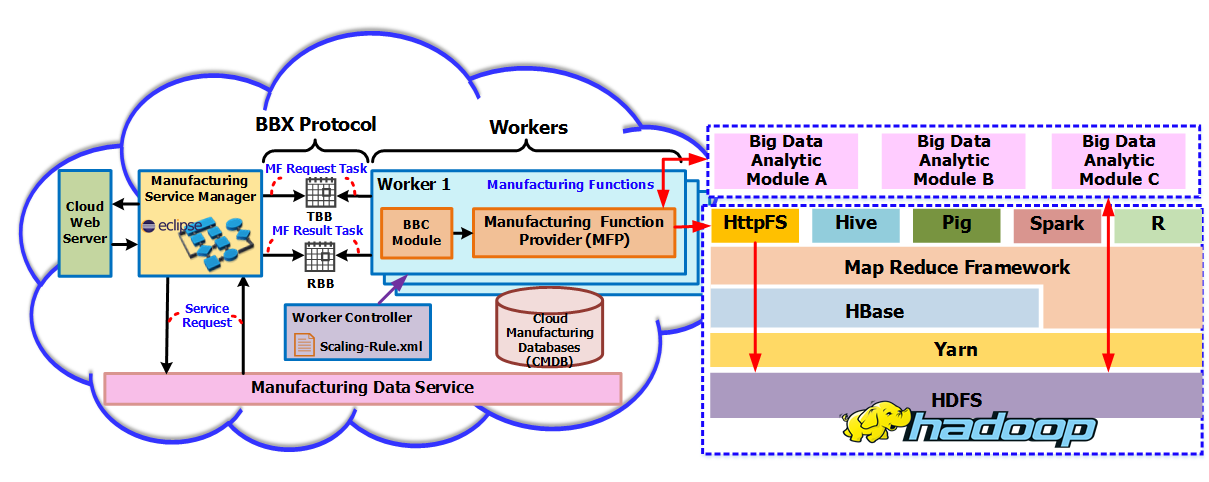
\includegraphics[scale=0.5]{figs/bda-cmfas.png}
				\caption{BDA-CMFAS 架構圖}
				\label{bda1}
			\end{center}
		\end{figure}

		整體架構如Figure. \ref{bda1}所示,我們將於Workers部分新增一個Manufacturing Function,其為一專門進行BDA服務呼叫之函數。它橋接了CMFAS與Hadoop系統,將透過以下步驟進行處理:
		\begin{enumerate}
			\item Manufacutring Function將欲處理之資料透過HttpFS送至HDFS中
			\item Manufacutring Function透過發送http需求來執行所定義好的BDA Function
			\item BDA Function自HDFS撈取所要處理的資料
			\item BDA Function進行運算後將結果回傳Manufacturing Function
			\item Manufacturing Function 將結果回傳至 BBC Module
		\end{enumerate}

		BDA Function除了可以使用原生之JAVA進行開發,也將可以採用R、Hive、Pig、Spark等程式進行開發,降低分散式程式開發的門檻,提升整體系統的生產力。

		企業選擇使用了CMFAS架構做為整個製造系統的核心,讓整套系統具有非常彈性化調整的空間,再加上了我們橋接了Hadoop運算平台以此來面對日益龐大的分析資料,結合了兩者的特性即可以為企業提供一個完美的雲製造系統。

\end{CJK*}
\end{document}